\section{Chronologie}
\label{sec:chronologie}

	Cette séparation des tâches nous a permis de réaliser un diagramme de Gantt du projet, avec des ressources affectées pour chaque tâche. Retranscrire exactement le diagramme de Gantt ne rendrait pas celui-ci très lisible, nous avons donc réalisé grâce à l'outil disponible sous Microsoft Project une frise chronologique qui reprend dans les grandes lignes ce dernier. Celui-ci est cependant disponible en annexe pour voir la liste entière de toutes les tâches du projet.

	Comme annoncé dans les rapports précédents, l'effectif de notre groupe pour la phase de conception et pour la phase de développement se voit réduit, puisqu'il ne restera plus que Marlène, Alexandre et Romain; les autres membres du groupe partant en semestre à l'étranger. Nous avons planifier l'estimation des tâches en prenant en compte cette réduction des ressources. Nous avons considéré 8h de travail par semaine par membre du projet (hormis les semaines réservées au projet, la semaine de partiel et les semaines de vacances), ceci sans compter les heures des réunions prévues chaque Mercredi. Cela représente donc 24h de travail effectif par semaine normale.

	Nous avons fixé la date de commencement de la phase de pré-développement au 16 janvier; les deux semaines précédentes étant consacrées aux révisions des partiels. La date de livraison finale est fixée au 27 mai. Cette livraison comprendra tous les rapports, les transparents des soutenances, les sources commentées, la documentation, les tests, une procédure d'installation et une machine virtuelle contenant la plateforme installée ainsi que tous les outils nécessaires. Ainsi, la durée entre le début de la phase de conception et la livraison finale est de 18 semaines.

	Les livraisons intermédiaires, quantàelles, sont déterminées à partir du temps de développement des fonctionnalités spécifiques à celles-ci. Ces dates, présentes dans la chronologie que vous pouvez retrouver plus bas, pourront donc légèrement ver suivant les retour que l'on recevra à chaque livraison. 

	D'un côté, un document Microsoft Project, qui a permis la génération du diagramme de Gantt, de la planification et de la chronie, smis à jour au fur et à mesure du développement pour suivre celui-ci dans le temps et s'assurer que les possibles retards n'impactent pas sur les livraisons ou sur le développement des fonctionnalités. D'un autre côté, un suivi des différentes tâches, permettant de suivre en détail les activités de chaque développeur 



	\begin{figure}[H]
        \centering
        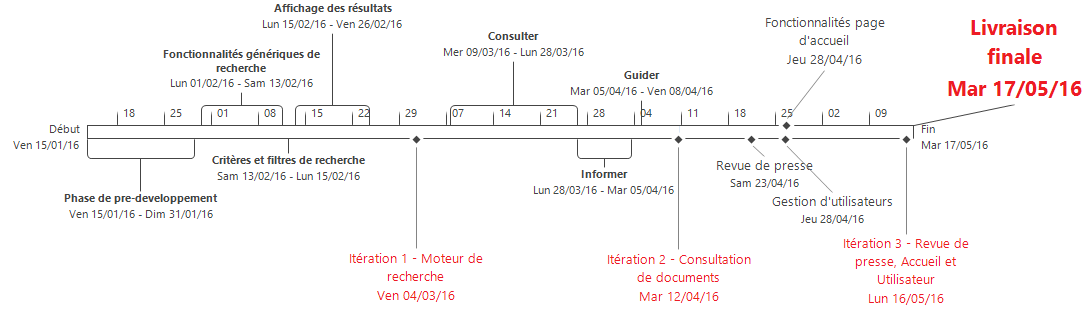
\includegraphics[width=1.3\textwidth, angle=90]{figure/frise.png}
            \caption{Frise chronologique représentant l'ensemble de la planification}
            \label{fig:frise}
    \end{figure}
